\section{EFP graf}
Predzadnji graf, ki sem ga risal je bil EFP graf.
\begin{figure}[h]
    \begin{center}
        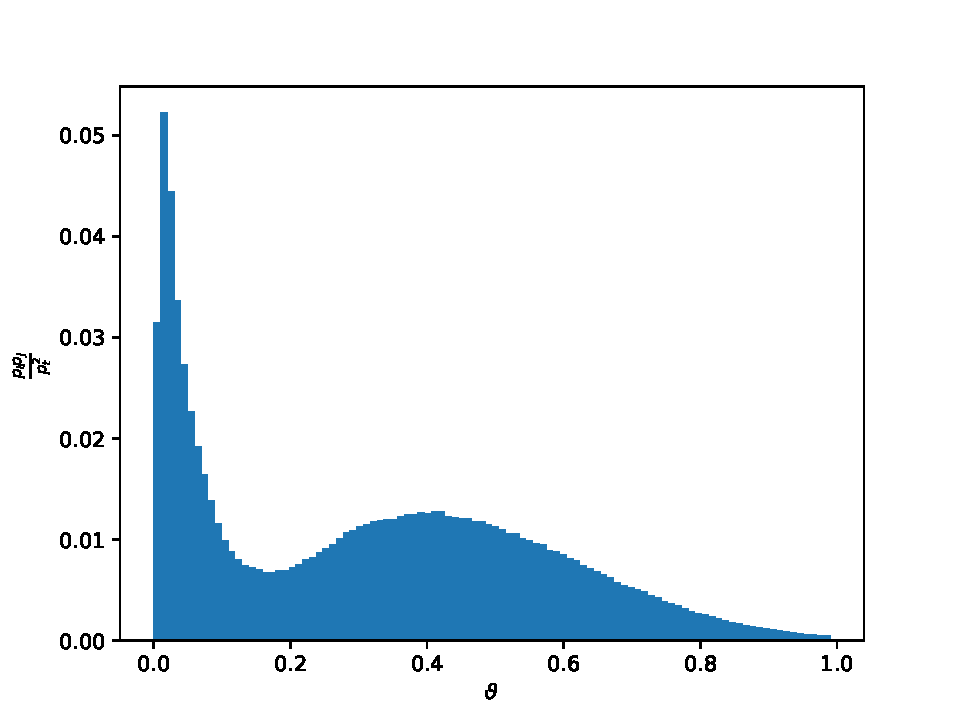
\includegraphics[width=13cm]{sections/section4/figures/ERPG_2_TTBar.pdf}
        \caption{Graf EFP}
        \label{slika 6}
    \end{center}
\end{figure}
\\
Kot je vidno iz slike, imamo dimenzijo $\vartheta$ in $\frac{p_ip_j}{p_T^2}$.
Spremenljivka $p_T$ predstavlja transverzalno gibalno količino danega jeta, $p_i$ pa
transverzalno gibalno količino delca v danem jetu.
\\
\\
Poglejmo si, kako se izračuna $\vartheta$.
\begin{equation}
    \vartheta_{ij}^2 = \left(\eta_i - \eta_j\right)^2+\left(\phi_i - \phi_j\right)^2
\end{equation}
Spremenljivki $\vartheta$ sem dopisal indekse, da je bolj očitno, iz katerih dveh
delcev $i$ in $j$ je izračunana. Podobno kot prej je treba graf normalizirat s številom
jetov, ki je bil risan. Pomembno je vedeti, da delca $i$ in $j$ pripadata istemu jetu.
\\
\\
Koda, ki izriše graf je v \verb|MAIN/main.py|, funkcije in grafi so pa iz moje strani 
poimenovani \verb|ERPG|. Zato tudi v kodi obstaja funkcija \verb|ERPG_2()|.